\section{Offline Trajectory Synthesis}
\label{sec:trajectory_synthesis}

The core idea of \model is to replace the costly iterative use of live search APIs with a locally served search engine, while retaining the noise and ambiguity inherent in real-world web research. We organize the pipeline into three stages: collecting challenging questions (\S\ref{subsec:qa_collection}), constructing an offline corpus with one-time online bootstrapping to ensure coverage (\S\ref{subsec:offline_search}), and synthesizing long-horizon trajectories with a teacher model in the offline environment (\S\ref{subsec:browser_tools}--\S\ref{subsec:trajectory_generation}).
Figure~\ref{fig:pipeline} provides a high-level overview of the pipeline.

\begin{figure*}[t]
    \centering
    % \vspace{-1em}
    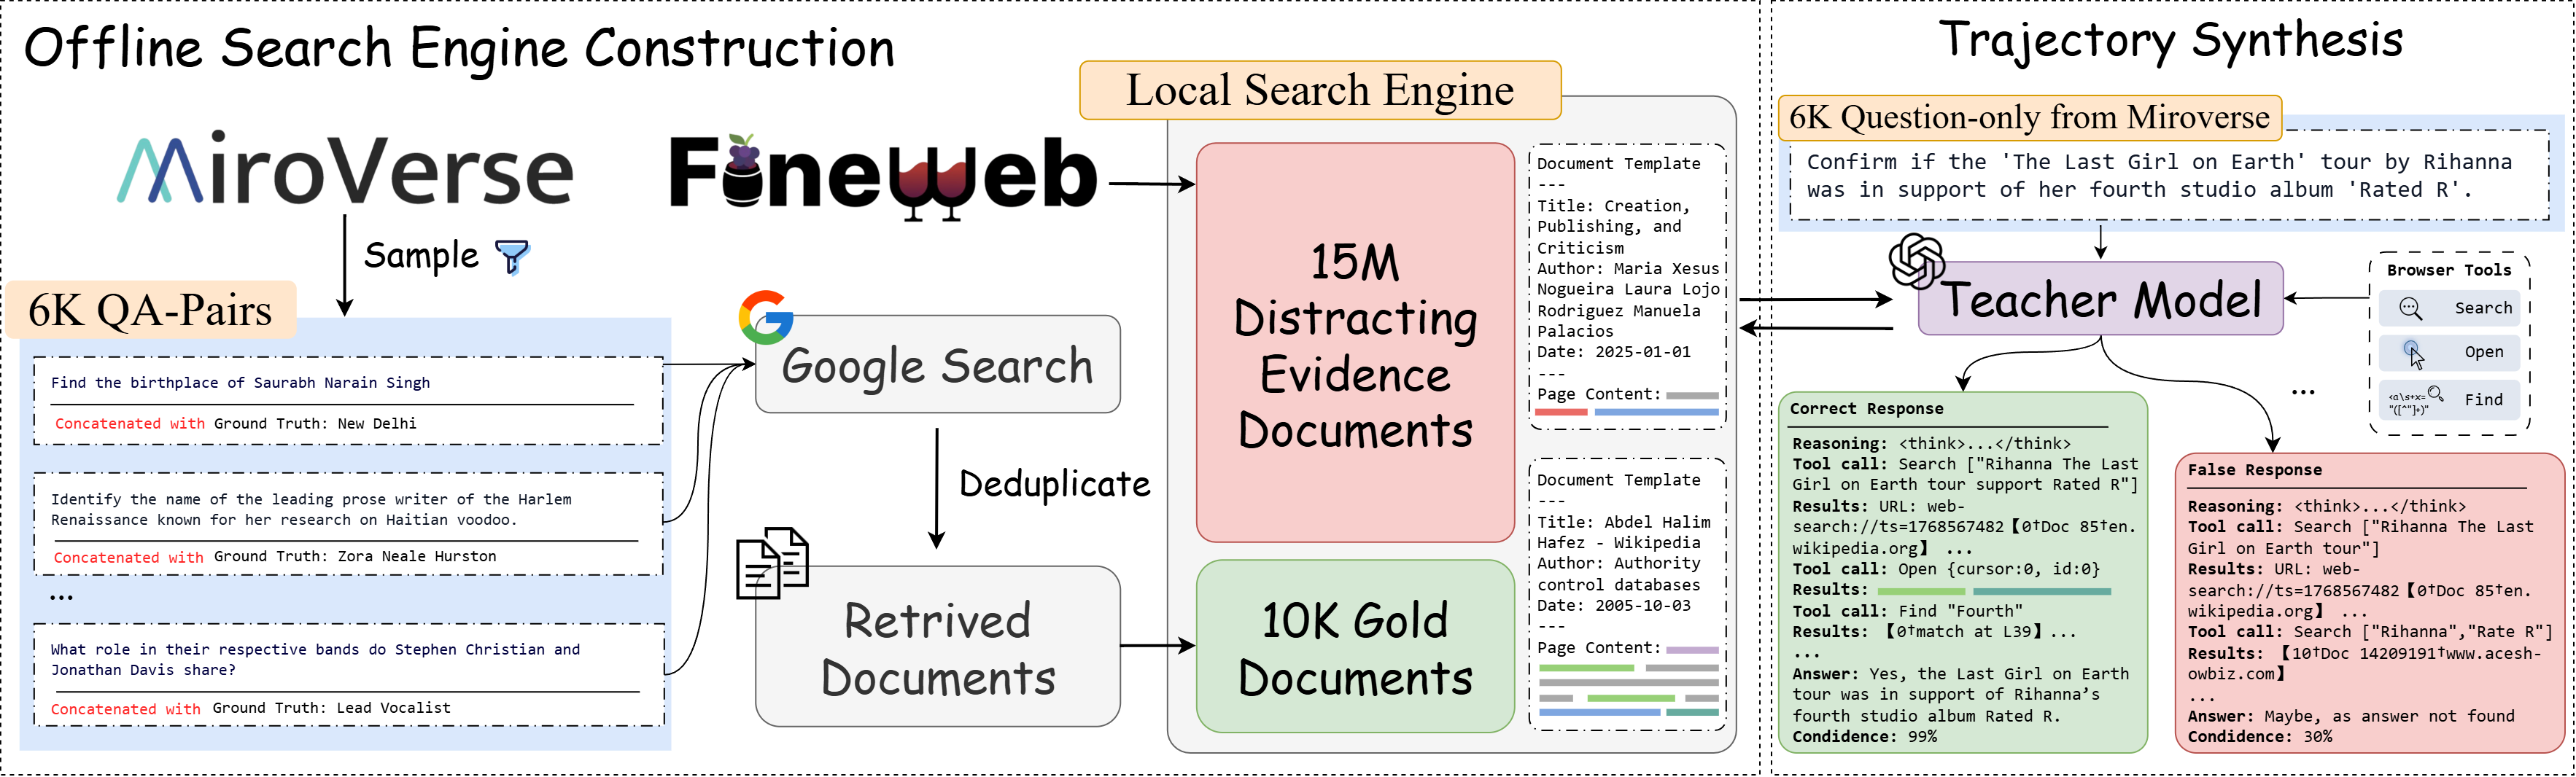
\includegraphics[width=0.99\textwidth]{img/Openresearcher-synthesis-v5.png}
    \caption{Overview of the \model trajectory synthesis pipeline. 
    (1) Curate challenging QA questions from MiroVerse; 
    (2) Construct an offline corpus by merging 15M FineWeb documents with 10K gold documents retrieved via one-time online bootstrapping; 
    (3) Built on this corpus,  a teacher model equipped with three browser primitives (\texttt{search}, \texttt{open}, and \texttt{find}) generates long-horizon trajectories in the offline environment.}
    \vspace{-1em}
    \label{fig:pipeline}
\end{figure*}

\subsection{QA Question Collection}
\label{subsec:qa_collection}

Synthesizing meaningful deep research trajectories requires questions that cannot be solved via shallow retrieval. 
Standard benchmarks such as 2WikiMultiHopQA~\citep{ho2020wikipedia} and NQ~\citep{kwiatkowski2019natural} are poorly suited for this purpose: most questions can be answered within 2--5 retrieval steps, and evidence is typically clear, well-structured, and densely cross-linked. In contrast, real deep research operates under web-scale complexity: reasoning often spans long-horizon, interdependent chains, while evidence is fragmented across heterogeneous sources and may be outdated or contradictory. 

To this end, we select questions from MiroVerse-v0.1~\citep{miromind2025mirothinker}, a dataset that explicitly requires long-horizon, multi-hop reasoning over heterogeneous evidence. 
Empirically, we observe that even a strong teacher model often needs dozens of tool calls in a search-augmented setting, with a substantial tail exceeding 100 calls.
From the full dataset, we randomly sample 10\% of the question--answer pairs, yielding roughly 6K QA instances. We then post-process each instance to normalize the answer into a concise, verifiable form (details in Appendix \S\ref{app:answer}).


Although MiroVerse provides partial trajectories, they are unsuitable for direct supervision: retrieved evidence may not support the final answer, search traces are often short or degenerate, and tool-use patterns vary widely across datasets. To synthesize high-quality, long-horizon research trajectories, we therefore regenerate all trajectories from scratch using only clean question–answer pairs. 



\subsection{Offline Search Engine Construction}
\label{subsec:offline_search}
Trajectory regeneration requires a simple prerequisite: \textit{the relevant evidence must be retrievable}. Otherwise, a failed trajectory is ambiguous: it may reflect a poor search strategy or simply missing evidence in the corpus. To reduce this ambiguity, we construct the offline search engine with explicit coverage-oriented bootstrapping prior to trajectory synthesis.


\paragraph{Gold Document Retrieval via Online Bootstrapping.}
To ensure corpus coverage, we perform answer-guided online bootstrapping to collect gold documents for each of the 6K QA pairs. (Gold documents refer to documents that collectively contain sufficient evidence to derive the ground-truth answer, either explicitly or implicitly.) This step is executed once during corpus construction and is not used during subsequent trajectory synthesis.
For each question, we: 
(1) construct the search query by concatenating the question and reference answer to improve recall~\citep{azad2019query};
(2) retrieve web content via the Serper API~\citep{serperdev2026}; 
(3) clean and deduplicate documents to remove boilerplate and non-content text. In total, we extract 10K gold documents for 6K questions.

\paragraph{Offline Corpus Construction.}
To approximate real-world web coverage and reflect realistic search complexity, we collect 15 million documents ($\approx$10 trillion tokens) from FineWeb~\citep{penedo2024fineweb}. These documents are merged with gold documents to form our offline corpus, where FineWeb documents act as distractors and gold documents provide answer-supporting evidence.

% \paragraph{Offline Corpus Construction.}
% To approximate real-world web-style coverage and reflect realistic search complexity, we collect 15 million documents ($\approx$10 trillion tokens) sampled from FineWeb~\citep{penedo2024fineweb}. These documents are merged with the gold documents to form our offline corpus, where FineWeb documents act as distractors and gold documents provide answer-supporting evidence.


\paragraph{Corpus Indexing.}
For efficient large-scale dense retrieval, each document is embedded using Qwen3-Embedding-8B~\citep{qwen3embedding} and indexed with FAISS~\citep{douze2024faiss}. 
At inference time, the agent issues natural-language queries, and the retriever returns ranked documents---simulating a web search API. Additional details on corpus indexing are provided in \S\ref{app:corpus_index}.


\begin{figure*}[t]
    \centering
    % \vspace{-1.5em}
    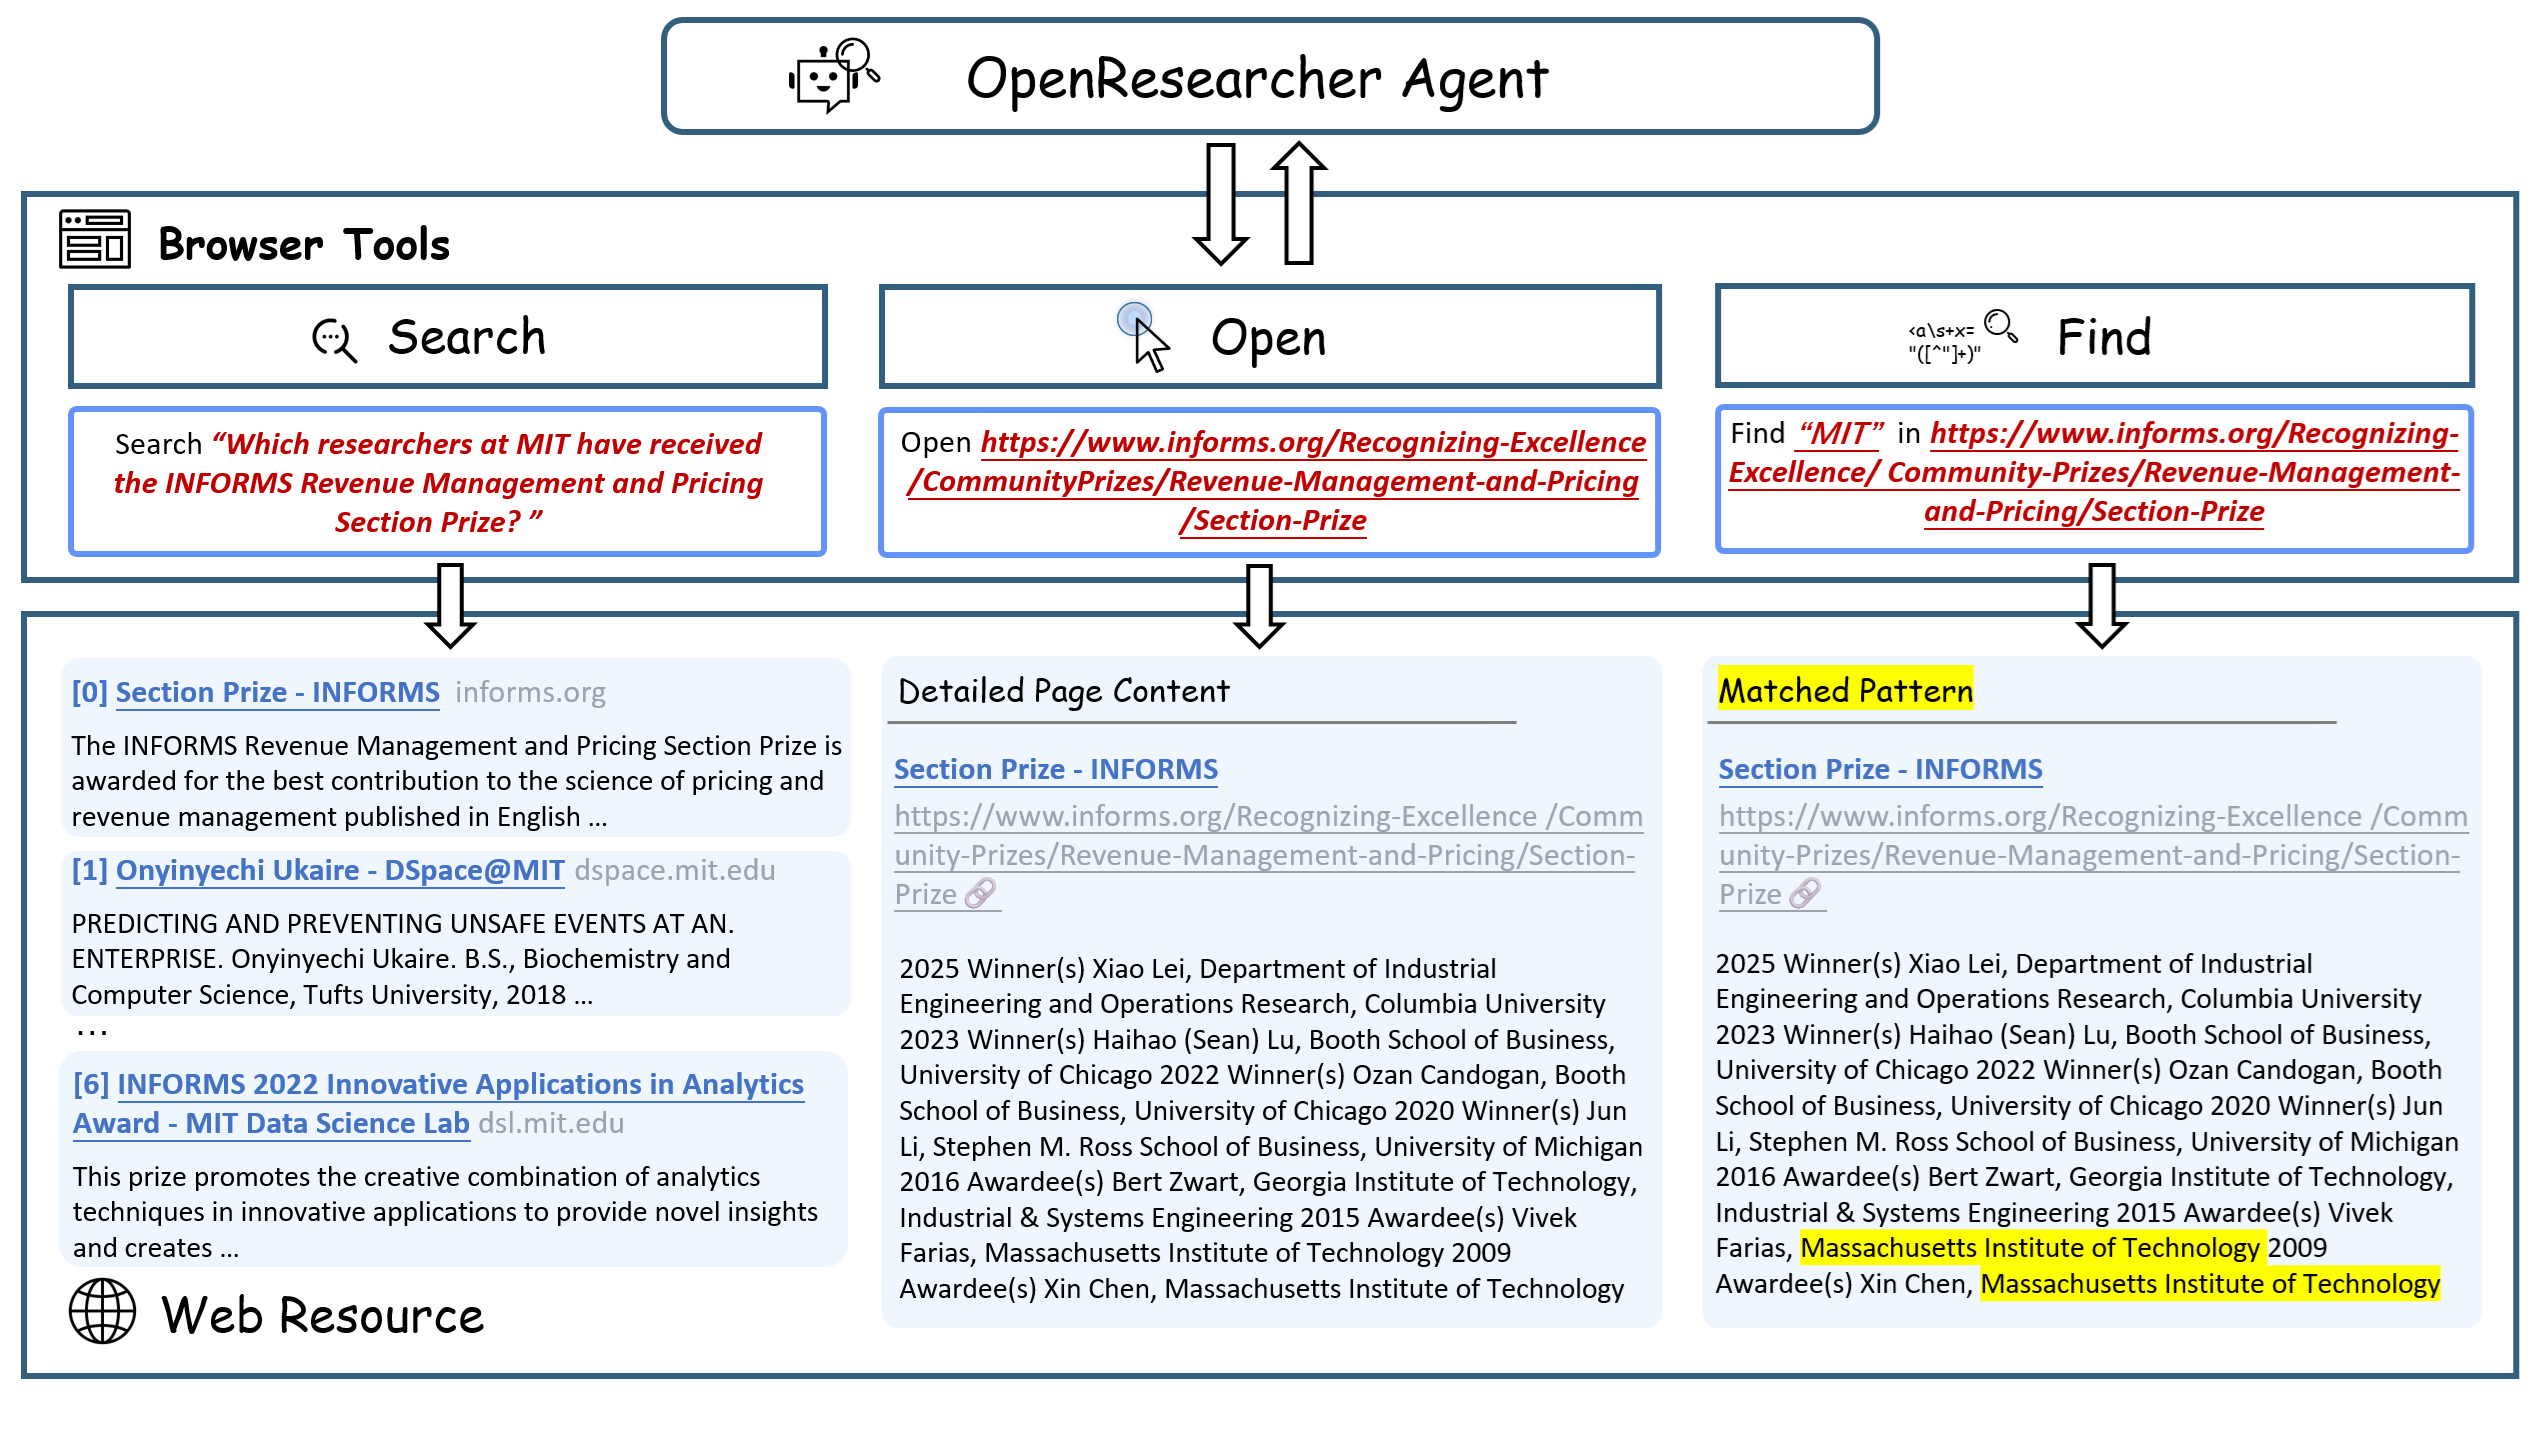
\includegraphics[width=0.98 \textwidth]{img/tools.png}
    \vspace{-0.5em}
    \caption{Overview of \model's browsing mechanism. The agent leverages three browser tools--\texttt{search}, \texttt{open}, and \texttt{find}--to interact with the web, progressively from retrieving search snippets to opening full pages and finally locating specific evidence within documents (e.g., identifying “MIT” in the page text), thereby enabling multi-scale information discovery.
    }
    \vspace{-1em}
    \label{fig:tools}
\end{figure*}


\subsection{From Search to Real Browsing}
\label{subsec:browser_tools}

Most prior agentic search systems~\citep{jin2025search, jiang2025verltool, li2025agentflow} treat search as a simple document retrieval operation: a query is issued, one or a few search snippets are returned, and reasoning proceeds directly over the retrieved content. However, this abstraction struggles with deep research questions that require iterative search, heterogeneous evidence aggregation, and long-horizon reasoning. Moreover, it differs substantially from how humans conduct research, which typically involves: (1) issuing a broad query to identify candidate sources; (2) opening promising documents to inspect their full content; (3) skimming, scrolling, and locating specific passages relevant to a working hypothesis; and (4) refining the query based on partial evidence and iterating.

To enable long-horizon deep research in a reproducible offline setting, we model browsing explicitly by exposing a minimal set of operations that support evidence discovery, verification, and synthesis. As shown in Figure~\ref{fig:tools}, we define three such primitives, each implemented as a corresponding tool:

\begin{itemize}[leftmargin=*, label=\textbullet]
    \item \texttt{Search}: Returns the top-$K$ results for a given query, each with a title, URL, and snippet (short excerpt from the document). This enables broad information retrieval to identify candidate sources.
    
    \item \texttt{Open}: Fetches the full content of a document from a URL. This mirrors the human act of clicking into a webpage to inspect it beyond search snippets.
    
    \item \texttt{Find}: Locates exact string matches within the currently opened document. This operation is critical for named-entity lookup, factual verification, and grounding intermediate hypotheses in concrete textual evidence.
\end{itemize}


These tools progressively narrow the agent’s focus from the corpus to documents and finally to evidence. Consequently, different tool sets enable information discovery at different scales. More concretely, search-only agents rely on incomplete snippets, whereas \texttt{search+open} still requires the model to implicitly scan long documents within the context window. The full \texttt{search+open+find} suite enables explicit evidence localization and better reflects real browsing behavior. We revisit this effect in the ablation study RQ$4$ (\S\ref{subsec:ablation}).


% \zhuofeng{I think we can delete this last paragraph.}

Building on these primitives, we leverage GPT-OSS-120B~\citep{agarwal2025gpt}---integrated with the browser tools and interacting with our offline search engine---to synthesize scalable, long-horizon deep research trajectories. Detailed agent prompts and tool metadata can be found in \S\ref{app:prompts}.

\subsection{Trajectory Generation Procedure}
\label{subsec:trajectory_generation}

With the offline corpus and browser tools in place, we synthesize trajectories by prompting the teacher model to: (1) use only the provided tools (\texttt{search}, \texttt{open}, \texttt{find}); (2) reason step-by-step before each tool call; and (3) terminate only when confident in a final answer. Crucially, the teacher model does not have access to the reference answer during generation and must recover it through multi-round search and reasoning.

We apply lightweight filtering to remove trajectories that: (1) exceed the maximum context length; (2) contain malformed tool calls; or (3) fail to reach a conclusive answer within the interaction budget. After filtering, we obtain \textbf{97K+ trajectories} spanning a broad range of reasoning horizons, including many cases exceeding 100 tool calls.
These trajectories serve as the foundation for post-training smaller reasoning models via supervised fine-tuning, as described in \S\ref{sec:exp-setup}. Implementation details are provided in Appendix \S\ref{app:synthesis}.

